\begin{abstract}
Compressed LoRA can outperform standard LoRA with far fewer trainable parameters. Low-dimensional adaptation can preserve useful capacity, but capacity alone does not determine when restricting estimation improves generalization. We develop a bias--variance account of compressed LoRA that connects this statistical question to compression geometry. Under a local quadratic approximation, restriction exchanges estimation variance for task-dependent projection bias. An isotropic sequence model yields an exact condition: compression helps a fixed task when its residual energy per excluded dimension is below the effective estimation noise; an additional isotropic target average gives an ensemble condition. The analysis predicts success and failure regimes as sample size, noise, and residual geometry vary. Projection-blind sequence experiments verify the exact crossover, and a nonlinear Transformer teacher--student study tests its qualitative persistence. Real-model diagnostics reveal variance reduction and task-dependent bias recovery, while delimiting the sample-size prediction. As a constructive consequence, an equal-budget analysis motivates Projected LoRA with Sparse Adapter (ProLoSA), which restores informative residual directions. Language understanding, mathematical reasoning, and instruction-tuning experiments assess its practical benefits and limits. Together, these results provide a statistical explanation of compressed adaptation and a design principle for correcting its recoverable bias.
\end{abstract}

\section{Introduction}
Low-Rank Adaptation (LoRA) \citep{hu2022lora} fine-tunes a frozen model through trainable low-rank factors. Compressed variants further restrict these parameters through sharing or fixed reconstructions, as in Tied-LoRA, VeRA, and Uni-LoRA \citep{renduchintala2024tied,kopiczko2024vera,li2025unilora}. Related structured PEFT methods such as FourierFT learn a small set of spectral coefficients for weight updates \citep{gao2024fourierft}. These methods show that substantial reductions in trainable parameters can preserve downstream performance. More surprisingly, some compressed configurations outperform standard LoRA. This raises a statistical question: \emph{when and why does compression make LoRA better, and when does that benefit disappear?}

Low intrinsic dimension motivates adaptation with few degrees of freedom \citep{aghajanyan2021intrinsic}. Existing explanations for Uni-LoRA, FourierFT, VB-LoRA, VeRA, and LoRA-XS emphasize compact representations, parameter sharing, or subspace geometry \citep{li2025unilora,gao2024fourierft,li2024vb,kopiczko2024vera,balazy2025lora}. These accounts do not provide an explicit bias--variance comparison establishing when compression improves population risk over standard LoRA and when that advantage disappears.

We develop a bias--variance account of compressed LoRA to characterize this comparison. Viewing compression as restricted estimation, we decompose local excess risk into task-dependent projection bias and estimation variance. Compression improves generalization when the variance removed from excluded directions exceeds the signal lost there. The explanatory variables are therefore the interaction between the chosen subspace, the required update, and estimation noise. This account explains how reducing adaptation capacity can improve estimation, while also identifying why the same restriction can become harmful.

The theory makes the explanation quantitative. In an isotropic sequence model, compression helps exactly when the fixed task's residual energy per excluded dimension falls below the effective estimation noise. Under local asymptotic assumptions, the risk advantage takes the form $A_{\mathrm{var}}/n-B_{\mathrm{proj}}$, exposing how data abundance can reveal a projection-bias floor. Subspace alignment and residual concentration provide further distinctions that parameter count alone cannot express. We test these implications through projection-blind sequence estimation, a nonlinear Transformer teacher--student experiment, and real-model diagnostics. The controlled experiments recover the crossover and failure regimes; the real-model study identifies variance reduction and task-dependent bias recovery, with the scope of its sample-size evidence assessed in Section~\ref{main:real}.

The explanation also yields a constructive implication: when excluded task energy is concentrated, a small residual branch can recover bias efficiently. Our equal-budget analysis compares this recovery with the projected capacity displaced by allocating parameters to the residual. We instantiate the resulting criterion as \textbf{Pro}jected \textbf{Lo}RA with \textbf{S}parse \textbf{A}dapter (\textbf{ProLoSA}), using warmup sensitivity to select residual coordinates. Its support ablations and downstream results test whether the statistical explanation leads to a useful adaptation design.

\paragraph{Contributions.}
\textbf{(i) A statistical explanation of compressed LoRA:} a local bias--variance decomposition linking compression geometry to the relative risk of compressed and full-space estimation.
\textbf{(ii) Testable success and failure conditions:} exact fixed-task and ensemble energy--noise thresholds, a conditional sample-size prediction, and mechanism tests spanning sequence models, a Transformer block, and real fine-tuning.
\textbf{(iii) Theory-guided bias correction:} an equal-budget residual-recovery criterion and its ProLoSA implementation, evaluated through support ablations and downstream benchmarks.

\subsection{Related Work}
Our statistical analysis builds on restricted-estimation and projection-risk methods \citep{maillard2009compressed,kaban2014new,thanei2017random}. Intrinsic-dimension research also provides compression-based generalization bounds \citep{aghajanyan2021intrinsic}; our object is the risk difference between a chosen compressed estimator and the full LoRA estimator, including the bias cost of excluding task directions. The fixed reconstruction directly models our Uni-LoRA branch; FourierFT restricts weight updates in a different coordinate space. LoRA expressivity \citep{zeng2024expressive}, optimization landscapes \citep{liu2025landscape}, gradient matching \citep{wang2025lorapro}, transformation-invariant optimization \citep{yen2025lorarite}, and feature-learning stability \citep{wu2026stablelora} address complementary questions. SparseAdapter and RoSA \citep{he2022sparseadapter,nikdan2024rosa} motivate comparison with sparse/hybrid adaptation; ProLoSA targets the bias induced by an additional compression constraint. Appendix~\ref{app:related} details these distinctions.

\section{When Does Compression Help?}
\label{main:theory}
\subsection{Restricted estimation and local risk}
Let $\theta\in\mathbb R^D$ collect the vectorized LoRA factors of the adapted layers. Standard LoRA estimates all $D$ entries; the compressed branch uses $\theta=Pz$, where $P\in\mathbb R^{D\times d}$ is fixed and $d\ll D$. Let $R(\theta)$ be population risk, $\theta^\star$ its full-space optimum, and $\theta_U^\star$ its optimum over $\operatorname{col}(P)$. Locally,
\begin{equation}
 R(\theta)-R(\theta^\star)\approx\tfrac12\|\theta-\theta^\star\|_H^2,
 \qquad H=\nabla^2R(\theta^\star)\succeq0.
 \label{main:quadratic}
\end{equation}
This is a neighborhood approximation, not global convexity. For estimators centered at their respective population optima, with covariances $\Sigma_L$ in the full space and $\Sigma_z$ in latent coordinates, the expected excess risks satisfy
\begin{align}
 \mathcal E_L&\approx\tfrac12\operatorname{tr}(H\Sigma_L),\nonumber\\
 \mathcal E_U&\approx
 \underbrace{\tfrac12\|\theta_U^\star-\theta^\star\|_H^2}_{B_{\mathrm{proj}}}
 +\underbrace{\tfrac12\operatorname{tr}(HP\Sigma_zP^\top)}_{V_U}.
 \label{main:decomp}
\end{align}
Thus compression helps when $B_{\mathrm{proj}}<\mathcal E_L-V_U$. Fewer parameters alone do not establish this inequality. Appendix~\ref{app:general_bias_variance} includes nonzero estimation and optimization bias; the derivation and definitions are in Appendix~\ref{sec:bias_variance}.

\subsection{An exact energy--noise condition}
Fix $\theta^\star$ and an orthonormal-column $P$, with $0<d<D$. In the sequence model, $y=\theta^\star+\sigma_{\mathrm{eff}}\epsilon$, $\epsilon\sim\mathcal N(0,I_D)$, and excess risk is $\frac12\|\theta-\theta^\star\|_2^2$. The estimators are $\hat\theta_L=y$ and $\hat\theta_U=PP^\top y$.
\begin{proposition}[Fixed-task and ensemble energy--noise conditions]
\label{prop:energy_noise}
Writing $q=(I-PP^\top)\theta^\star$, expectation over observation noise gives
\begin{equation}
 \mathcal E_L=\tfrac12D\sigma_{\mathrm{eff}}^2,\qquad
 \mathcal E_U=\tfrac12\|q\|_2^2+\tfrac12d\sigma_{\mathrm{eff}}^2.
 \label{main:sequence}
\end{equation}
Compression helps this fixed task if and only if
\begin{equation}
 \hat v_\perp:=\frac{\|q\|_2^2}{D-d}<\sigma_{\mathrm{eff}}^2.
 \label{main:threshold}
\end{equation}
If targets are additionally generated independently of $P$ with mean zero and covariance $vI_D$, then $\mathbb E\|q\|^2=(D-d)v$ and the ensemble-average condition is $v<\sigma_{\mathrm{eff}}^2$.
\end{proposition}
The proof is in Appendix~\ref{app:energy_noise_condition}. Repeated datasets for one task average over observation noise, not over target generation; their threshold uses $\hat v_\perp$. When noise decreases, a nonzero residual produces a bias-dominated regime. The scalar energies depend on the chosen coordinates: LoRA's rescaling $(A,B)\mapsto(cA,B/c)$ preserves $BA$ but changes factor norms. Accordingly, the isotropic threshold applies within a fixed parameterization; real-model diagnostics use predictive quantities or curvature-weighted residual energy.

\subsection{Sample size and residual recovery}
For a regular fixed-dimensional M-estimator in an identifiable tangent space, a shared-local approximation to the full and restricted Hessians and score covariances gives
\begin{equation}
 \Delta(n):=\mathbb E[R(\hat\theta_L)-R(\hat\theta_U)]
 \approx A_{\mathrm{var}}/n-B_{\mathrm{proj}}.
 \label{main:sample}
\end{equation}
Let $G=\operatorname{Cov}(\nabla_\theta\ell)$ be the per-example score covariance at $\theta^\star$. In identifiable coordinates, the shared-local approximation yields
\begin{equation}
 A_{\mathrm{var}}=\tfrac12\left[\operatorname{tr}(H^\dagger G)
 -\operatorname{tr}\!\left((P^\top HP)^\dagger P^\top GP\right)\right]\ge0,
 \label{main:avar}
\end{equation}
where ${}^\dagger$ denotes inversion on the identifiable tangent space. The inequality follows by projecting the positive-semidefinite whitened score covariance onto a subspace. It does not require the information-matrix identity $G=H$. The full sandwich-covariance derivation is in Appendix~\ref{sec:testable_predictions}.

If both coefficients in Eq.~\eqref{main:sample} are positive, $n^\star=A_{\mathrm{var}}/B_{\mathrm{proj}}$ predicts a crossover; if $B_{\mathrm{proj}}=0$, no finite crossover is required. This large-$n$ approximation need not hold with high-dimensional estimation, early stopping, or different local geometries. Noise that increases score covariance without moving the optimum increases the predicted compression advantage. Better subspace alignment helps when the accompanying variance change is controlled; equal dimension alone is insufficient under anisotropic curvature.

\paragraph{What can be falsified?}
Holding the task and training protocol fixed, the local model predicts a nonnegative slope in $1/n$ and a nonpositive large-$n$ intercept for $\Delta(n)$. A variance-reduction signature alone cannot verify both terms. Label perturbations test the noise prediction only when they preserve the population optimum; arbitrary label flipping need not do so. The controlled sequence and Transformer experiments probe the crossover and failure regimes, while the real-model study tests the sample-size signature and decomposes predictive variability directly.

\begin{proposition}[Matched-budget residual correction]
\label{prop:matched_budget}
Under the ensemble model of Proposition~\ref{prop:energy_noise}, compare a target-independent $B$-dimensional compressed space with a hybrid $\operatorname{col}([P,E_I])$ of rank $B$, where $d=B-K$ and $E_I$ selects $K$ coordinates. Assume support selection is independent of estimation noise. Define $A_I=(I-PP^\top)E_I$, $q=(I-PP^\top)\theta^\star$, and $\mathcal E_K=\|\Pi_{A_I}q\|^2$, where $\Pi_{A_I}$ is the orthogonal projector onto $\operatorname{col}(A_I)$. Then
\begin{equation}
 \mathbb E[R(\hat\theta_{\mathrm{hyb}})-R(\hat\theta_{U,B})]
 =\tfrac12(Kv-\mathbb E[\mathcal E_K]).
 \label{main:matched}
\end{equation}
Both estimators have variance $B\sigma_{\mathrm{eff}}^2/2$, so the hybrid wins exactly when $\mathbb E[\mathcal E_K]>Kv$.
\end{proposition}
Appendix~\ref{app:matched_budget} proves the result. Target-independent supports have no expected gain; concentrated residual energy permits informed correction, whereas diffuse energy limits it. Actual warmup selection uses the estimation data and violates the independence assumption. Its extra selection variance and noisy energy estimates can offset bias recovery; the proposition therefore supplies a design criterion, not a guarantee for trained ProLoSA.

\section{ProLoSA: Sparse Residual Correction}
\label{main:method}
ProLoSA allocates $B=d+K$ trainable parameters between a compressed latent vector $z$ and sparse coefficients $\alpha$:
\begin{equation}
 \theta_D=Pz+R\alpha,\qquad R=[e_{i_1},\ldots,e_{i_K}].
 \label{main:method_eq}
\end{equation}
We use Uni-LoRA's normalized one-hot reconstruction $P$ \citep{li2025unilora}: each full-space coordinate is assigned to one latent coordinate, and each column is normalized to unit norm. The fixed projection ties coordinates globally; the routed residual provides selected local corrections. Reconstructed entries are unpacked into standard LoRA factors, whose updates can be merged into the frozen backbone.

Training has two stages. First, only $z$ is optimized. After a score-free warmup, a fixed scoring window accumulates the SNIP-style sensitivity \citep{lee2018snip}
\begin{equation}
 s_i=\sum_{t\in\mathcal T_{\mathrm{score}}}|\theta_{D,i}^{(t)}g_i^{(t)}|,
 \qquad g^{(t)}=\nabla_{\theta_D^{(t)}}\mathcal L^{(t)}.
 \label{main:snip}
\end{equation}
Second, we select the top-$K$ coordinates, initialize $\alpha=0$, and jointly train $z,\alpha$ with $P,R$ fixed. Zero initialization preserves the current prediction when the branch activates. SNIP measures local sensitivity rather than the unknown residual energy in Proposition~\ref{prop:matched_budget}; its usefulness is tested empirically. Appendix~\ref{app:method_details} gives the projection, the score-free warmup plus 128-step scoring schedule, and Algorithm~\ref{alg:prolosa}.

\section{Testing the Mechanism}
\label{main:experiments}
We test three levels of the argument: the exact sequence-model threshold, qualitative behavior in a nonlinear Transformer, and statistical signatures in real fine-tuning. These mechanism checks use controlled comparisons within each experiment; the broader downstream benchmarks in Section~\ref{main:downstream} serve a separate practical purpose.

\subsection{Projection-blind sequence estimation}
\label{main:synthetic}
We draw one target independently of the compression projection and fix both across 200 observation-noise trials. A heavy-tailed mixture gives concentrated residual energy; a dense Gaussian target gives a diffuse failure regime. With $D=4096$ and $n_{\mathrm{eff}}=512$, observation noise is $\sigma_{\mathrm{eff}}=\sigma_y/\sqrt{n_{\mathrm{eff}}}$. Figure~\ref{main:fig_sequence} compares compressed-only dimension $B=48$ with hybrids of $d=16$, $K=32$. Hybrid supports are random, target-informed top-$K$ residual (oracle), or noisy-residual top-$K$, the sequence analog of warmup selection. Complete generation and estimation protocols are in Appendix~\ref{sec:synthetic}.

\begin{figure}[t]
 \centering
 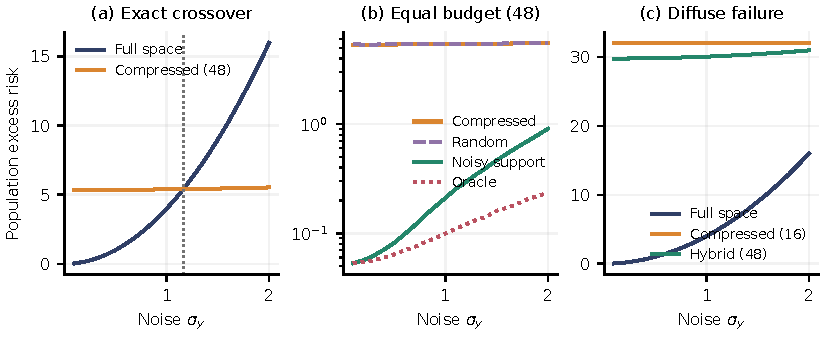
\includegraphics[width=\linewidth]{figures/sequence_summary.pdf}
 \caption{\textbf{Sequence-model tests.} (a) Full-space and compressed risk cross near the fixed-instance prediction $\sigma_y^\star\approx1.16$ (dashed). (b) At equal budget $B=48$, informed supports improve on compression; random support tracks it. (c) A dense target defeats both compression ($d=16$) and the larger hybrid ($d+K=48$) throughout the tested range. This last panel tests failure, not equal-budget superiority. Each target and its projections are fixed across the 200 noise trials and all noise levels; full decompositions are in Appendix~\ref{app:mechanism}.}
 \label{main:fig_sequence}
\end{figure}

The observed crossover agrees with the realized residual-energy threshold, rather than requiring an average over tasks. At matched budgets, random support approximately ties pure compression, while informed supports recover much more bias. The noisy support separates from the oracle as noise grows, exposing the cost excluded by the idealized independence assumption. In the diffuse regime the compressed bias floor is about $32$, above full-space LoRA across the tested range, and sparse correction recovers little. The original $d=16$ versus $d+K=48$ comparison and all decompositions remain in Appendix~\ref{sec:synthetic}; they illustrate bias recovery but are not evidence for equal-budget superiority.

\subsection{From the sequence model to a Transformer}
\label{main:transformer}
We pretrain and freeze a Transformer block of width 64 and sequence length 32, then plant query/value weight updates and fit noisy teacher outputs with AdamW. Compression and routing act in the identifiable $8192$-dimensional weight-update space, rather than the bilinear LoRA-factor coordinates. We compare rank-4 LoRA (1024 parameters), compressed-only adaptation ($B=128$), and hybrids ($d=K=64$), together with full updates and oracle/random supports. Thus this is a nonlinear bridge experiment, not an identical parameterization to every real-model run. We report excess prediction MSE, without the sequence model's factor $1/2$. The concentrated and diffuse teachers have functional displacements of $10\%$ and $100\%$, respectively; they vary magnitude as well as concentration. Appendix~\ref{sec:transformer_synthetic} specifies the construction and controls.

\begin{figure}[t]
 \centering
 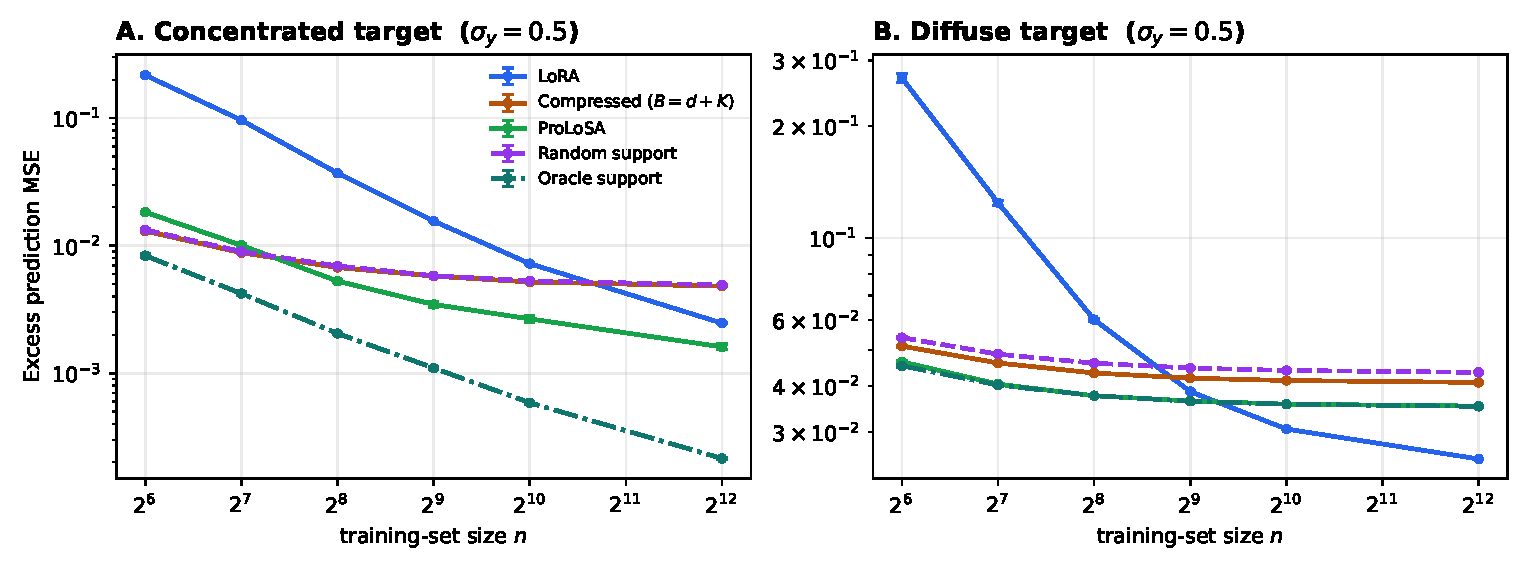
\includegraphics[width=\linewidth]{transformer_risk_vs_n.pdf}
 \caption{\textbf{Transformer teacher--student prediction MSE versus sample size.} Concentrated and diffuse targets, $\sigma_y=0.5$; mean $\pm$ s.e. over 20 training seeds for each fixed teacher. LoRA overtakes compression with more data. Sparse correction helps for concentrated residuals but little for diffuse residuals, even with oracle support. Compressed-only and all hybrids share budget 128. Additional noise levels and function-space decompositions are in Appendix~\ref{sec:transformer_synthetic}.}
 \label{main:fig_transformer}
\end{figure}

At $\sigma_y=0.5$, LoRA crosses below matched-budget compression around $n=2^9$--$2^{10}$ for the diffuse target and $n=2^{11}$ for the concentrated target (Figure~\ref{main:fig_transformer}). Higher noise shifts the crossover toward larger $n$. Noiseless large-sample fits show compressed approximation floors of $0.0047$ and $0.041$, respectively; oracle correction removes $99\%$ of the concentrated floor but only $13\%$ of the diffuse floor. Within each fixed teacher, function-space decompositions show the transition from high variance to a compressed bias floor; the two teachers are evaluated separately.

The finite-training deviations are also informative. At $n=4096$, $\sigma_y=1$, ProLoSA improves concentrated-target risk from $0.0052$ to $0.0030$, but at $n=64$, $\sigma_y=1.5$, noisy warmup selection worsens it from $0.066$ to $0.105$. Random hybrids do not outperform equal-budget compression and can be slightly worse under anisotropic curvature. These observations support residual recovery while delimiting the idealized variance equality in Proposition~\ref{prop:matched_budget}.

\subsection{Mechanism tests in real fine-tuning}
\label{main:real}
We next examine RoBERTa-large with rank-4 LoRA as a full-factor-space baseline and matched trainable budgets for Uni-LoRA and ProLoSA. Each comparison shares data subsets and evaluation sets; settings and full results are in Appendix~\ref{sec:real_model_validation}. We use dev loss for sample-size scaling, predictive probabilities for empirical decomposition, and diagonal empirical-Fisher weighting for residual diagnostics. These measurements address distinct parts of the argument and do not assume that raw factor norms measure functional error.

\begin{figure}[t]
 \centering
 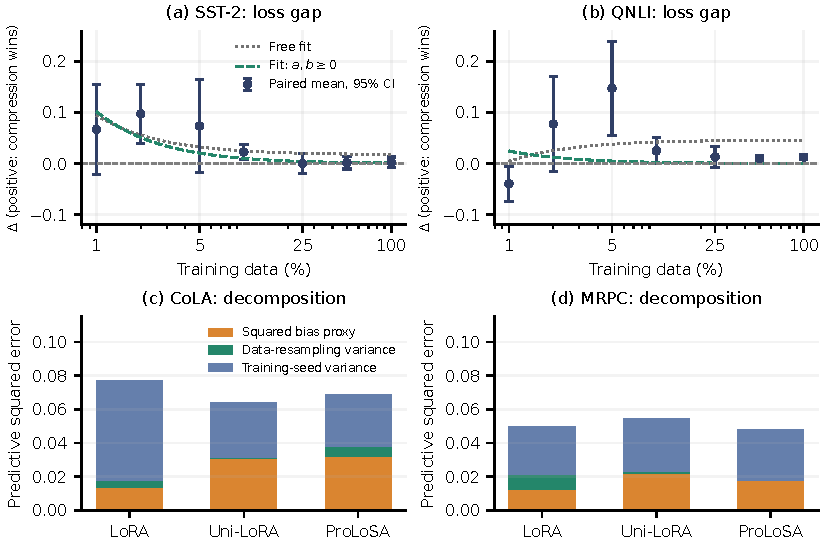
\includegraphics[width=\linewidth]{figures/real_mechanism.pdf}
 \caption{\textbf{Real-model evidence and limits.} Top: paired dev-loss gaps $\Delta=L_{\mathrm{LoRA}}-L_{\mathrm{Uni}}$ with pointwise 95\% $t$ intervals over five training seeds and free/constrained $a/n-b$ fits; positive favors compression. Subsets are fixed across seeds. Bottom: squared bias proxy, data-resampling variance, and training-seed variance, shown separately for five resamples and two seeds. The reference is a full-data LoRA ensemble; Table~\ref{tab:e3_reference} checks its sensitivity.}
 \label{main:fig_real}
\end{figure}

\paragraph{Sample-size scaling.}
We vary the training fraction from $1\%$ to $100\%$ with a fixed update-step budget and five paired training seeds, keeping the subset fixed at each fraction. SST-2's mean gap contracts from $0.067$ (95\% interval $[-0.021,0.155]$) to $0.002$ ($[-0.008,0.013]$). Fitting these paired means gives $\hat a=52.14$, $\hat b=-0.0171$, $R^2=0.485$; imposing $a,b\geq0$ places $b$ at zero and lowers $R^2$ to $0.358$. QNLI's free slope is negative ($\hat a=-43.90$, bootstrap interval $[-63.14,-29.14]$), and the auxiliary CoLA mean curve has $R^2=0.014$. These deviations challenge the local sample-size model under the present training protocol; they cannot be attributed solely to an unobserved crossover. Appendix~\ref{sec:real_model_validation} reports paired intervals, fit residuals, and uncertainty.

\paragraph{Predictive bias and variance.}
Five 80\% data resamples and two training seeds per resample separate data-resampling variability from within-resample variability, including initialization, optimization, and the compressed projection seed. On CoLA, Uni-LoRA lowers total variance from $0.0636$ to $0.0332$, but $88\%$ of this reduction comes from the training-seed component ($0.0593\to0.0326$), rather than the data component ($0.0043\to0.0006$). Thus the total decrease is not a measurement of $A_{\mathrm{var}}/n$. Squared bias relative to a full-data LoRA ensemble rises from $0.0136$ to $0.0309$. On MRPC, ProLoSA lowers Uni-LoRA's bias proxy from $0.0219$ to $0.0180$, with no increase in total variance; CoLA lacks this correction. Both bias orderings persist with rank-4-only, rank-64-only, and leave-one-reference-out ensembles. Finite-replicate corrections and clipping are detailed in the appendix.

\paragraph{Sparse recoverability.}
From an explicitly full-data, multi-seed LoRA target proxy, we form the Euclidean residual $q_E=(I-PP^\top)\Delta\theta$ and measure coordinate capture $\rho_{I,H}^2=\sum_{i\in I}\hat H_{ii}q_{E,i}^2/\sum_i\hat H_{ii}q_{E,i}^2$ using a diagonal empirical Fisher. Uniform size-$K$ support samples from all $D$ original coordinates, so its expected capture is $K/D$. The saved full-data SNIP supports show $16$--$194\times$ enrichment (Table~\ref{main:tab_recovery}), corroborated by 10,000 random supports per task. This coordinate diagnostic differs substantially from projection-bias recovery: on MRPC, capture is $18.04\%$ on $q_E$, $2.67\%$ on the $\hat H$-orthogonal residual, and joint refitting recovers $5.68\%$ of the latter's weighted energy. These are distinct proxies; none directly measures the unknown population quantity in Proposition~\ref{prop:matched_budget}. The support ablation below tests practical selection performance.

\begin{table}[t]
 \centering\small
 \caption{\textbf{Residual coordinate-energy capture.} Fisher-weighted fractions on the Euclidean residual of a full-data target proxy; enrichment uses $K/D$. Budgets, saved-support provenance, and the geometry comparison appear in Appendix~\ref{sec:real_model_validation}.}
 \label{main:tab_recovery}
 \begin{tabular}{lrrrr}
 \toprule
 Task & Oracle & SNIP & Reference & Enrichment \\
 \midrule
CoLA & 49.87\% & 7.91\% & 0.4883\% & $16.21\times$ \\
MRPC & 69.45\% & 18.04\% & 0.4883\% & $36.94\times$ \\
QNLI & 14.46\% & 3.12\% & 0.0407\% & $76.52\times$ \\
RTE & 33.74\% & 1.14\% & 0.0407\% & $27.98\times$ \\
STS-B & 51.91\% & 7.91\% & 0.0407\% & $194.13\times$ \\
 \bottomrule
 \end{tabular}
\end{table}

\section{Downstream Performance and Ablations}
\label{main:downstream}
Table~\ref{main:tab_performance} summarizes practical results; Appendix~\ref{app:downstream} contains all baselines, task-level scores, and hyperparameters. GLUE averages improve from $85.3$ to $85.5$ on RoBERTa-base and $88.3$ to $88.7$ on RoBERTa-large at the same compressed budget, while full LoRA remains stronger on the base-model average. Changing backbones changes representation quality and curvature as well as dimension, so this comparison is not a controlled variance test.

\begin{table}[t]
 \centering\small
 \caption{\textbf{Downstream summary.} Parameters are trainable counts. GLUE averages six tasks (five seeds); full task-level uncertainty and baseline provenance appear in Table~\ref{tab:glue}. Mathematical reasoning reports GSM8K / MATH (Gemma) or MATH500 (Llama); full comparisons are in Table~\ref{tab:math}. $^\dagger$VB-LoRA uses the original paper's parameter-count convention. Llama results use one seed and post-hoc compressed-configuration selection.}
 \label{main:tab_performance}
 \begin{tabular}{llrl}
 \toprule
 Backbone & Method & Parameters & Score(s) \\
 \midrule
 RoBERTa-base & LoRA & 0.295M & 86.6 \\
 & Uni-LoRA / ProLoSA & 0.023M & 85.3 / 85.5 \\
 RoBERTa-large & LoRA & 0.786M & 87.8 \\
 & VeRA & 0.061M & 87.8 \\
 & VB-LoRA & 0.162M$^\dagger$ & 88.2 \\
 & LoRA-XS & 0.025M & 87.9 \\
 & Uni-LoRA / ProLoSA & 0.023M & 88.3 / 88.7 \\
 \midrule
 Gemma-7B & LoRA & 200M & 74.90 / 31.28 \\
 & VeRA & 1.90M & 74.98 / 28.84 \\
 & FourierFT & 0.59M & 72.97 / 25.14 \\
 & Uni-LoRA & 0.52M & 75.59 / 28.94 \\
 & ProLoSA & 0.52M & 74.69 / 29.90 \\
 Llama-3.1-8B & LoRA ($r=64$) & 167.77M & 79.61 / 33.20 \\
 & Uni-LoRA & 1.05M & 75.44 / 26.20 \\
 & ProLoSA & 1.05M & 75.06 / 26.60 \\
 \bottomrule
 \end{tabular}
\end{table}

On mathematical reasoning, ProLoSA improves Gemma-7B's MATH score over Uni-LoRA by $0.96$ points but loses $0.90$ on GSM8K. Llama-3.1-8B similarly gains $0.40$ on MATH500 and loses $0.38$ on GSM8K; both compressed methods remain below rank-64 LoRA. These Llama results use seed 42, and the displayed compressed configurations maximize each method's two-benchmark mean among available runs at that budget: they are a post-hoc test-set summary, not an independently selected validation result (Appendix~\ref{app:llama31_math_sweep}). Each model is trained once on MetaMathQA and evaluated on both benchmarks, so their score differences cannot identify task-specific training-update energies. Instruction-tuning results are in Table~\ref{tab:instruction}; for example, LLaMA2-13B MT-Bench single-/multi-turn scores rise from $6.34/4.43$ to $6.57/4.72$ under a shared 1.0M budget.

\begin{table}[t]
 \centering\small
 \caption{\textbf{Vision transfer with ViT-B/16.} Final-model accuracy (\%, seed 42). All methods use rank 4 and train the classification head; adapter budgets exclude this shared head: LoRA has 147,456 parameters and both compressed methods have 24,600 ($d+K$ for ProLoSA). Parentheses give $d:K$. All four ratios are shown; no best-epoch or best-ratio selection is applied. Appendix~\ref{app:vit} gives exact budgets, settings, and the 72,000-budget sweep.}
 \label{tab:vit}
 \setlength{\tabcolsep}{5pt}
 % Generated from final_accuracy, seed 42; do not edit.
\begin{tabular}{lrrrrr}
\toprule
 & \multicolumn{3}{c}{1,000 training images} & \multicolumn{2}{c}{CIFAR-100} \\
\cmidrule(lr){2-4}\cmidrule(lr){5-6}
Method & CIFAR-100 & Food-101 & DTD & 5,000 & Full \\
\midrule
LoRA ($r=4$) & 86.91 & 79.50 & 73.14 & 89.87 & 92.41 \\
Uni-LoRA & 86.59 & 79.25 & 72.66 & 89.55 & 92.10 \\
ProLoSA ($2:1$) & 86.35 & 79.26 & 72.71 & 89.13 & 92.03 \\
ProLoSA ($4:1$) & 86.50 & 79.10 & 72.29 & 89.32 & 92.33 \\
ProLoSA ($8:1$) & 86.34 & 79.19 & 72.50 & 89.28 & 92.02 \\
ProLoSA ($12:1$) & 86.39 & 79.25 & 72.71 & 89.36 & 91.99 \\
\bottomrule
\end{tabular}

\end{table}

\paragraph{Vision transfer.}
Following Uni-LoRA's ViT experiments \citep{li2025unilora}, we evaluate ProLoSA on ViT-B/16 with shared data subsets and equal compressed-adapter budgets (Table~\ref{tab:vit}). At $d:K=4:1$, ProLoSA improves full-data CIFAR-100 accuracy from Uni-LoRA's $92.10$ to $92.33$, while LoRA reaches $92.41$. Gains are not consistent: all four allocations trail Uni-LoRA on CIFAR-100 with 1,000 and 5,000 images, and differences on Food-101 and DTD are small. These single-seed results extend the allocation study to vision without establishing a general advantage or a sample-size crossover; the training horizon also changes across data sizes.

\begin{table}[H]
 \centering\small
 \caption{\textbf{Equal-budget ablations}, $d+K=23040$. CoLA: Matthews correlation; MRPC: accuracy, mean $\pm$ std. Hybrid supports share $d=22320$, $K=720$. Full allocation and warmup sweeps are in Table~\ref{tab:ablation_budget_full}.}
 \label{main:tab_ablation}
 \begin{tabular}{lcc}
 \toprule
 Variant & CoLA & MRPC \\
 \midrule
 Compressed-only & $68.99\pm0.58$ & $90.93\pm0.00$ \\
 Sparse-only & $59.99\pm1.40$ & $84.89\pm0.83$ \\
 Random-support hybrid & $66.58\pm0.63$ & $90.28\pm0.61$ \\
 Gradient-support hybrid & $67.95\pm0.59$ & $90.03\pm0.31$ \\
 SNIP-support hybrid & $69.62\pm1.84$ & $91.69\pm0.40$ \\
 \bottomrule
 \end{tabular}
\end{table}

At a fixed total budget, SNIP support outperforms random and accumulated-gradient supports on both ablation tasks (Table~\ref{main:tab_ablation}); pure sparsity performs substantially worse. Random support also trails pure compression in the real network, unlike the idealized isotropic tie. The evidence favors informed residual allocation while retaining the practical effects of curvature, conditioning, and selection noise.

\section{Discussion and Conclusion}
\label{sec:conclusion}
This work develops a bias--variance explanation of compressed LoRA: its statistical advantage is governed by the balance between removed estimation variance and excluded task signal. The resulting conditions connect subspace geometry, noise, and sample size to beneficial and harmful compression, and motivate ProLoSA as a correction for recoverable projection bias under a fixed budget. Controlled and real-model experiments examine both the explanation and its design consequence. The exact thresholds belong to the sequence model; real-task sweeps do not establish a reliable crossover, and optimization effects or noisy support selection can alter the trade-off. These boundaries specify where further validation and theory are needed.
